\section{\texorpdfstring{Relativní vyčíslitelnost}{Relativní vyčíslitelnost}}
\vspace{5mm}
\large

Zobecnění 1-převoditelnosti na relativný výpočet (s Orákulem).

\begin{definition}[tt-Převoditelnost]
	Tzv tt (truth table) převoditelnost znamená, že existuje $f \in ORF$ která vrátí:
	\[ x \to
		\left\{
		\begin{array}{lll}
			n_x \\
			\alpha_x & \text{n-arní booleovskou funkci} \\
			y_1, \ldots, y_n & \text{body}
		\end{array}
		\right.
	\]
	Pro niž platí:
	\[ C_A(x) = \alpha_x(C_B(y_1), \ldots, C_B(y_n))\]
	Kde $C_i$ je charakteristická funkce.

	Neboli
	\[ x \in A \iff \alpha_x(\ldots) = 1 \]

	Značení:
	\[ A \leq_{tt} B \]
\end{definition}

\begin{note}
	TT převoditelnost musí napřed říct, na které body se bude ptát.
	Což je omezení.
\end{note}

\subsection{Formalizace relativního vypočtu}

Existuje několik možnosti formalizace:
\begin{definition}[Formalizace relativního vypočtu]
	\begin{enumerate}
		\item TS s orákulem. Přidáme další pasku, kde TS bude umisťovat slova pro dotazy k orákulu.
			Pak množina $B$ (asi jazyk orákula) je dalším vstupem programu.
		\item ČRF. Přidáme charakteristické funkce $C_B$, kde $B$ je proměnná.
		\item Programovací jazyk. Přidáme funkci $B$, v console se objeví dotaz, jestli slovo patří nebo nepatří do jazyka.
	\end{enumerate}
\end{definition}

\begin{note}
	Relativní výpočet je jedním z druhu paralelizace.
	Pro konkretní vstup $x$ vzniká tzv výpočtový strom.

	Důležité je, že množina konečných větví je r.s.
	Každou z větvi lze charakterizovat pomoci
	\[ \langle x, v, y, n \rangle \]
	Kde $x$ je vstup, $v$ je vystup, $y$ je index konečné množiny kladně zodpovězených orákulem dotazů, $n$ je index množiny negativních dotazů.
	Přitom
	\[ D_y \subseteq B, D_n \subseteq \overline{B} \]

	Předpokládáme, že jazyk orákula je korektní, neboli
	\[ D_y \cap D_n = \emptyset \]

	Tento přistup formalizace není nejvýhodnější, protože body na které se ptáme netvoří souvislý počátek přirozených čísel.
\end{note}

\begin{agreement}[Strings]
	Nadále pracujeme s konečné binární řetízky (string), které značíme buď $\{ 0, 1 \}^{\ast}$, nebo $2^{<w}$.

	Operace:
	\begin{itemize}
		\item konkatenace: $\sigma * \tau$.
		\item délka: $|\sigma|$
		\item indexovaní: $\sigma(0) * \sigma(1) * \ldots * \sigma(|\sigma| - 1)$.
		\item počátek(ostrý): $\alpha \preccurlyeq \beta (\alpha \prec \beta)$.
		\item počátek množiny: $\alpha \prec B$ což znamená $\alpha \preccurlyeq C_B$.
	\end{itemize}
\end{agreement}

\begin{definition}[Částečně rekurzívní funkcionál]
	Částečně rekurzívní funkcionál je r.s. množina $\Phi$ trojic taková, že pokud platí:
	\begin{gather*}
		\langle \sigma, x, y \rangle \in \Phi \\
		\langle \sigma^{\ast}, x, y^{\ast} \rangle \in \Phi \\
		\sigma \preccurlyeq \sigma^{\ast}
	\end{gather*}
	Tak $y = y^{\ast}$.

	Funkcionál je funkce vyššího řadu, vrací funkce.
\end{definition}
Q: co přesně znamená $y^{\ast}$.

\begin{note}
	Přístupy jsou ekvivalentní, protože v případě Částečně rekurzívního funkcionálu číslo na které se orákula neptáme označíme nulou v řetízku.
\end{note}

\begin{example}
	Program má na vstupu $x$, na vystup vypíše $y$ s použití $\alpha \preccurlyeq B$.
\end{example}

\begin{definition}[ČRF-nál zobrazení]
	Částečně rekurzívní funkcionál určuje částečné zobrazení:
	\begin{gather*}
		\Phi(\sigma)(x) \simeq y \iff \langle \sigma, x, y \rangle \in \Phi \\
		\Phi(\tau)(x) \simeq y \iff \text{pro nějaké}\ \sigma \preccurlyeq \tau: \Phi(\sigma)(x) \simeq y\\
		\Phi(B)(x) \simeq y \iff \text{pro nějaké}\ \sigma \preccurlyeq B: \Phi(\sigma)(x) \simeq y
	\end{gather*}
\end{definition}

Q: proč funkcionál místo zobrazení s 2ma parametry?

\begin{note}
	Máme funkcionální term, který aplikujeme na $0,1$ (charakteristickou) funkci.
	Tím dostaneme funkční term. Aplikace funkčního termu na číselný term může ale nemusí davat číselnou hodnotu.
\end{note}

\begin{properties}[Částečně rekurzívní funkcionál]
	\begin{enumerate}
		\item $\Phi(B)$ je korektně definováno.
		\item $\Phi(B)$ je intuitivně efektivně vyčíslitelné pomoci B.
			Postup: efektivně generuj trojice $\langle \sigma, x, y \rangle$.
			Pak $\sigma \prec B$? Pokud ano, stop.
			Jinak pokračuj dal.
		\item Výpočetní strom $\to \Phi$ vystihuje pojem efektivní vyčíslitelnosti vzhledem k $B$.
	\end{enumerate}
\end{properties}

\begin{definition}[T-Převoditelnost]
	\[ A \leq_T B \]
	Pokud existuje nějaký ČRFunkcionál $\Phi$:
	\[ \Phi(B) = A, \forall x( A(x) = \Phi(B)(x)) \]
	Taky se říká: A je B-rekurzívní, A je reflexivní vzhledem k B.
\end{definition}

\begin{definition}[T-Převoditelnost pro funkce]
	$\varphi$ je $B$-ČRF pokud
	\[ \varphi(x) \simeq \Phi(B)(x) \]
\end{definition}

\begin{lemma}[Regularizační funkce]\label{reg_func}
	Existuje ORF (dokonce PRF) $\rho$ regulárizační funkce.
	Splňující:
	\begin{enumerate}
		\item $W_{\rho(x)} \subseteq W_x$.
		\item $W_{\rho(x)}$ je ČRFunkcionál.
		\item $W_x$ je ČRFunkcionál $\Rightarrow W_{\rho(x)} = W_x$.
	\end{enumerate}
\end{lemma}
\begin{proof}
	Není formální důkaz.

	Budeme efektivně generovat $W_x$.

	\begin{enumerate}
		\item foreach($tmp = \langle \sigma, x, y \rangle \in W_x$)
		\item \tab if($W_{\rho(x), s} \cup \{tmp\}$ je regulární)
		\item \tab \tab $W_{\rho(x)} = W_{\rho(x)} \cup \{tmp\}$ //add
	\end{enumerate}
\end{proof}

\begin{definition}[Numerace funkcionálu]
	$W_{\rho(x)}$ z lemmatu je $e$-tý ČRF-nál, značíme $\Phi_e$.
	\[ \Phi_e(B)(x) \simeq y \iff \langle \sigma, x, y \rangle \in W_{\rho(x)}: \sigma \prec B \]
	Taky za s kroků: $\Phi_{e, s}(B)(x)$.
\end{definition}

\begin{observation}[ČRF-nál r.s.]
	$\Phi_e(\sigma)(X) \downarrow$ je r.s.

	$\Phi_{e, s}(\sigma)(X) \downarrow$ je rekurzívní.

	$\Phi_e(B)(X) \downarrow$ je r.s. v $B$.

	$\Phi_{e, s}(B)(X) \downarrow$ je rekurzívní v $B$.
\end{observation}

\begin{theorem}[s-m-n pro Relativní]\label{s_m_n_rel}
	% todo zneni
\end{theorem}
\begin{proof}
	%7. predn od 44:00
	Nemůžeme rovnou použit standardní s-m-n větu, protože ne každá $W_x$ splňuje funkční vlastnost.
	Proto potřebujeme Regularizační funkce \cref{reg_func}.

	Pak $\Phi_e(B)(x)$ je univerzální $B$-ČRF.
	Pak platí
	\[ \forall B, \forall x_1, \ldots, x_m, y_1, \ldots, y_n: \Phi_e(B)(x_1, \ldots, x_m, y_1, \ldots, y_n) \simeq \Phi_{\overline{s_m}(e, x_1, \ldots, x_m)}(B)(y_1, \ldots, y_n) \]
	Kde $\overline{s_m}$ jsou ORF (dokonce PRF).

	Formálně, uděláme ČRF takovou, že
	\[ \alpha(e, x, w) \downarrow \iff w = \langle \sigma, y, t \rangle: \langle \sigma, \langle x, y \rangle, t \rangle \in W_{\rho(x)} \]
	S tím, že
	\[ \alpha(e, x, w) \simeq \varphi_{s_2(a, e, x)}(w) \]
	Položme
	\[ \overline{s_2}(e, x) = s_2(a, e, x) \]

	Rozbor: s pomoci $\sigma$ orákulu a vstupu $y$ vypočti $t$ jestliže
	\[ \Phi_e(\sigma)(\langle x, y \rangle) = t \]
	Což znamená (pro jednoduchost pro 2 proměnné):
	\[ \Phi_e(B)(\langle x, y \rangle) \simeq \Phi_{\overline{s_2}(e, x)}(B)(y) \]
\end{proof}

\begin{properties}[Turingovská převoditelnost]
	\begin{enumerate}
		\item $\leq_T$ je reflexivní, tranzitivní.
		\item A rekurzívní $\Rightarrow \forall B: A \leq_T B$.
		Pokud umíme spočítat $A$, tak to můžeme udělat s libovolným orákulem bez dotazů.
		\item $B$ rekurzívní $\land A \leq_T B \Rightarrow A$ je rekurzívní.
			Pro dotazy k orákulu $B$ použijeme TS který rozhoduje $B$.
			Jako vnoření vypočtu v složitosti.
	\end{enumerate}
\end{properties}

\begin{definition}[Turingovská ekvivalence]
	\[ A =_T B \iff A \leq_T \land B \leq_T A \]
\end{definition}

\begin{definition}[T Stupně převoditelnosti]
	\[ deg_T(A) = \{ B: B \leq_T A \} \]
\end{definition}

\begin{note}
	$\{ \varphi_e \}_x$ a $\{ \Phi_e(\emptyset)(x) \}$ jsou různá vyjádření právě všech ČRF.
	Jsou rekurzivně izomorfní: máme efektivní překladač mezi těmito systémy.
\end{note}

\begin{definition}[B-rekurzívní spočetnost]
	A je $B$-r.s. právě když
	\[ A = dom(\Phi_e(B)) \]
\end{definition}

\begin{notation}[e-ta B-r.s. množina]
	\[ W^B_e = dom(\Phi_e(B)) \]

	Podobně za $s$ kroků:
	\[ W^B_{e, s} = dom(\Phi_e(B)) \]
\end{notation}

\begin{definition}[T-úplnost]
	A je $T$-úplná pravě když je r.s. a platí
	\[ \forall B \in r.s.: B \leq_T A \]

	Taky
	\[ A <_T B \iff A \leq_T B \land B \nleq_T A \]
\end{definition}

\subsection{Struktura T-stupňu}

\begin{definition}[T stupně struktura]
	T-stupně tvoří horní polosvaz (upper semilattice), označuji se $\mathcal{D}(\leq)$.

	Nechť $a, b$ třídy ekvivalence v $\mathcal{D}(\leq)$.
	Pak
	\[ a \leq b \iff \exists A \in a, \exists B \in b: A \leq_T B \]
\end{definition}

\begin{definition}[Join]
	\[ A \ \text{join}\ B = A \oplus B = \{ 2x: x \in A, 2x + 1: x \in B \} \]
\end{definition}

\begin{properties}[Join]
	\begin{itemize}
		\item $A \leq_T A \oplus B$.
		\item $B \leq_T A \oplus B$.
		\item $B \leq_T C \land A \leq_T C \Rightarrow A \oplus B \leq_T C$.
	\end{itemize}
\end{properties}

\subsection{Relativizace dřívějších výsledků}

\begin{observation}\label{rel_prop}
\begin{itemize}
	\item Postová věta:
		$A$ je $B$-rekurzívní $\iff A, \overline{A}$ jsou $B$-r.s.
	\item r.s. které mají enumerator jsou efektivně generovatelné.
		Podobně, $B$-r.s která má enumerator je efektivně generovatelná relativně k $B$.
	\item r.s. množiny jsou právě ty, které lze vyjádřit pomoci $\exists ($ rekurzívní podmínka $)$.
		Podobně: $B$-r.s. množiny jsou právě ty, které lze vyjádřit pomoci $\exists (B-$rekurzívní podmínka $)$.
\end{itemize}
\end{observation}

Q: co je $B$-rekurzívní podmínka? Zahrnuje taky $y \in B$?

\subsection{Operace skoku}

\begin{definition}[Jump]\label{jump}
	Skok neboli relativizovaný Halting problém.
	\[ A^{\prime} = \{ x: \Phi_x(A)(x) \downarrow \} = \{ x: x \in W_x^A \} \]
\end{definition}

\begin{theorem}[Vlastnosti skoku]
	\begin{enumerate}
		\item $A^{\prime}$ je r.s.
		\item $A^{\prime}$ není $A$-rekurzívní \& $\overline{A^{\prime}}$ není $A$-r.s.
		\item $B$ je $A$-r.s $\iff B \leq_1 A^{\prime}$.
		\item $B$ je $A$-r.s \& $A \leq_1 C \Rightarrow B$ je $C$-r.s.
		\item \[ A \leq_T B \iff A^{\prime} \leq_1 B^{\prime} \]
		\item \[ A \equiv_T B \iff A^{\prime} \equiv_1 B^{\prime} \]
	\end{enumerate}

	Kde $\equiv$ je znak rekurzívní izomorfie.
\end{theorem}
\begin{proof}
	\begin{enumerate}
		\item z definice, $A^{\prime}$ je definičním oborem programu $\Phi_x(A)(x)$.
		\item Cantorová diagonální metoda. Formálně:
			\[ \overline{A^{\prime}} = \{ x : x \notin W_x^A \} \Rightarrow \forall x: \overline{A^{\prime}} \neq W_x^A \]
			Pak z relativní Postové věty \cref{rel_prop}: $A^{\prime}$ není $A$-rekurzívní.
		% 8 predn od 41:00
		\item "$\Leftarrow$". Nechť $B \leq_1 A^{\prime}$.Pak
			\[ \exists f \in ORF: x \in B \iff f(x) \in A^{\prime} \]
			Z toho můžeme spočítat $f(x)$ a pokud $f(x) \in A$ tak $x \in B$.
			Což je program pro rozhodnutí $B$.

			"$\Rightarrow$" Pomoci fiktivní proměnné.
			Sestavíme
			\[ \alpha(x, y, w) \downarrow \iff y \in W_x \]
			Dle s-m-n věty \cref{s_m_n_rel}
			\[ \alpha(x, y, w) \simeq \varphi_{h(x, y)}(w) \]
			Dosadíme za fiktivní proměnnou $w = h(x, y)$.
			Pak
			\[ h(x, y) \in K \iff y \in W_x \]
			% todo nechapu tento krok, proč potřebujeme x_0??
			Zvolme $x = x_0$, pak $h(x_0, y)$ 1-převádí $W_x$ na $K$.

			V relativním případě máme $W_x^A$ a $A^{\prime}$ místo $K$.
		\item Když $B$ je $A$-r.s. a $A \leq_T C$. Víme:
			\[ B = dom(\Phi_e(A)) \]
			v průběhu vypočtu se objeví dotazy $z \in A$?
			Vnoříme pro každý dotaz proceduru, která rozhoduje $A$ pomoci $C$.
			Pak
			\[ B = dom(\Phi_i(C)) \]

			Pozor, důkaz není formální.
		\item Máme následující diagram:

		% obrazek, 18. lekce 51:00
		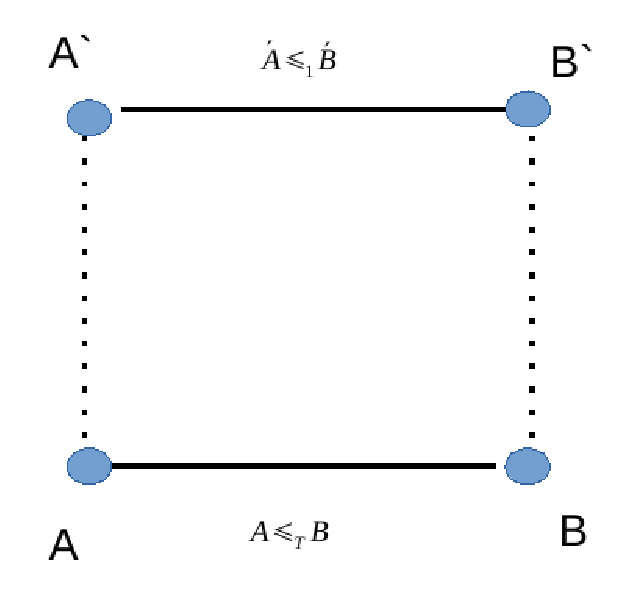
\includegraphics[scale=0.4]{skok_diag.eps}

		"$\Rightarrow$". Nechť $A \leq_T B$.
		Víme z 1), že $A^{\prime}$ je $A$-r.s.
		Podle 4) $A \leq_T B \Rightarrow A^{\prime}$ je $B$-r.s.
		Tedy dle 3) protože $B^{\prime}$ je "nejtěžší" mezí $B$-r.s (je 1-úplná pro $B$-r.s):
		\[ A^{\prime} \leq_1 B^{\prime} \]

		"$\Leftarrow$". Nechť $A^{\prime} \leq_1 B^{\prime}$.
		Triviálně: $A, \overline{A}$ jsou $A$-rekurzívní proto dle relativní Postové věty \cref{rel_prop}:
		$A, \overline{A}$ jsou $A$-r.s.

		Pak dle 3) $A^{\prime}$ je 1-úplná pro všechny $A$-r.s.
		\[ A, \overline{A} \leq_1 A^{\prime} \]
		Z předpokladu, relace je tranzitivní
		\[ A, \overline{A} \leq_1 B^{\prime} \]
		Proto $A, \overline{A}$ jsou $B$-r.s.
		Konečně dle relativní Postové věty \cref{rel_prop} $A$ je rekurzívní v $B$:
		\[ A \leq_T B \]

		\item Přímý důsledek 5), aplikujeme relaci na obou stranách.

	\end{enumerate}
\end{proof}

\begin{note}
	\[ deg_T(A) = \{ B: A \equiv_T B \} \]
	Se po skoku zobrazí na třídu 1-ekvivalence $A^{\prime}$.

	% todo obrazek predn 8 01:01:00
\end{note}

\begin{definition}[Jump na T-stupních]\label{jump_T}
	$\underline{a}^{\prime}$ skok T-stupně $\underline{a}$ je třída
	\[ \{ B: B \geq_T A^{\prime}, A \in a \} \]
	Na volbě $A$ nezáleží protože relace $\equiv_T$ je ekvivalence.
\end{definition}

\begin{note}
	Skok lze iterovat:
	\[ (A)^0 = A, (A)^{(n + 1)} = (A^{(n)})^{\prime} \]

	Taky všechny konečné:
	\[ A^{(\omega)} = \{ \langle x, y \rangle: x \in A^{(y)} \} \]

	Analogicky na třídách
	\[ \underline{a}^0 = \underline{a}, (\underline{a})^{(n + 1)} = (\underline{a}^{(n)})^{\prime} \]
\end{note}

\begin{observation}[$deg_T(\emptyset)$]
	\[ \underline{0} = deg_T(\emptyset) \]
	Což jsou právě všechny rekurzívní množiny.
\end{observation}

\begin{lemma}[$K$ a $\emptyset^{\prime}$]
	$K$ a $\emptyset^{\prime}$ jsou různá vyjádření Halting problému.
	Jsou rekurzivně izomorfní: máme efektivní překladač mezi těmito systémy.
\end{lemma}
\begin{proof}
	Protože $\emptyset^{\prime}$ je $\emptyset$-r.s. $\Rightarrow \emptyset^{\prime}$-r.s. $\Rightarrow \emptyset^{\prime}  \leq_1 K $.

	Opačně $K$ je r.s. (absolutně) $\Rightarrow \emptyset$-r.s. $\Rightarrow K \leq_1 \emptyset$.
\end{proof}

\subsection{Stejnoměrnost}
Tvrzení o skoku platí stejnoměrně (jako v analýze).

\begin{theorem}[Stejnoměrnost skoku]
	\[ \exists z_0 \forall A (W_{z_0}^A = A^{\prime}) \]
	Existuje pevný program, který funguje pro všechny množiny.
\end{theorem}
\begin{proof}
	\[ W_{z_0} = \{ \langle \sigma, x, y \rangle: \langle \sigma, x, y \rangle \in W_{\rho(x)} \} \]
	Pak $W_{z_0}$ je regulární, protože prvky bereme z regulární množiny $W_{\rho(x)}$.
	Dal
	\[ x \in A^{\prime} \iff \Phi_x(A)(x) \downarrow \iff \exists \sigma, \exists y(\langle \sigma, x, y \rangle \in W_{\rho(x)} \land \sigma \prec A) \iff x \in W_{z_0}^A \]

	Podobně: \[ \exists f \in ORF \forall A, B, \forall z: A = \Phi_z(B) \Rightarrow A^{\prime} \leq_1 B^{\prime}\ \text{pomoci}\ \varphi_{f(z)} \]
	Kde $\varphi_{f(z)}$ je ORF, prostá.
\end{proof}
